\documentclass[12pt]{article}

\usepackage{times}
\usepackage{amsmath}
\usepackage{latexsym}
\usepackage{fullpage}
\usepackage{graphicx}
\usepackage{amsfonts}

\graphicspath{ {./images/} }

\newcommand{\NOT}{\neg}
\newcommand{\AND}{\wedge}
\newcommand{\OR}{\vee}
\newcommand{\XOR}{\oplus}
\newcommand{\IMPLIES}{\rightarrow}
\newcommand{\IFF}{\leftrightarrow}
\newcommand{\E}{\exists}
\newcommand{\A}{\forall}

\setlength{\parskip}{.1in}

\renewcommand{\baselinestretch}{1.1}

\begin{document}

\begin{center}

{\bf
CSCE 313\\
PA3-Report\\
Jeffrey Xu\\
10/04/20\\
}

\end{center}

\section{Design}

Compared to PA1, this programming assignment makes significant changes to the types of IPC methods used to communicate between the server and client and the class design for implementing these forms of communication. Some changes to the number of channels that can be created has also been changed and the functionality of transferring files has changed. 

To begin, a base abstract class \emph{RequestChannel} was created to allow for abstraction of the different types of requests channels and allowed for polymorphic data structures. The abstract class has a virtual destructor, \emph{cread}, \emph{cwrite} and \emph{open\_ipc} functions. The \emph{cread} and \emph{cwrite} functions are pure virtual forcing the subclasses to implement them. The abstract class constructor also stores the two file descriptors and the name of the channel. 

For each different type of channel, the constructor will call the abstract constructor and initialize the name of each channel path (\emph{s1, s2}) along with calling \emph{open\_ipc} to initialize each file descriptor (except for shared memory). Each channel destructor also properly closed the file descriptor and cleaned up the memory associated with each form of IPC. Finally, the \emph{cread} and \emph{cwrite} methods use the IPC-specific functions to read and write from and to the IPC form of communication. 

Within the server/client code, more code was added to handle the \emph{-i} flag and add the functionality for more channels in client for \emph{-c} flag. The server and client also handled the \emph{-i} flag by using polymorphism on the \emph{RequestChannel} object to determine what type of channel to create. Also, the client coded has been adjusted to handle multiple channels. \emph{getnDataPointsFromVector} and \emph{getDataFromFileFromVector} were created to handle multiple channel requests. These functions work by looping through each channel in the passed in vector; requesting data points simply loop through each channel and performs the proper requests and for file requests, each channel writes only a segment of the file. As for remainder bytes, the code handles that by making the last channel write the extra bytes to the file. 

\section{Time Complexity}

For requesting the 1000 data points, the time needed for each channel types takes about 2.8 sec to 3.0 sec for all channel types. The times for each types of channel (running 5 channels) on one execution is shown below (order of pictures: FIFO, MQ, SHM). 

\begin{center}
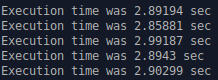
\includegraphics[width=5cm, height=2cm]{F_Time}\,
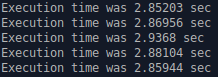
\includegraphics[width=5cm, height=2cm]{Q_Time}\,
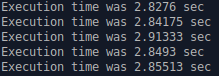
\includegraphics[width=5cm, height=2cm]{M_Time}
\end{center}

As for file requesting, there seemed to be some differences between the different channel types. For this test, a 100MB file was used. Some pictures showing the execution time for each type of channel used on this file is shown below.

\begin{center}
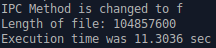
\includegraphics[width=5cm, height=1.2cm]{F_File}\,
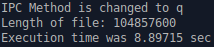
\includegraphics[width=5cm, height=1.2cm]{Q_File}\,
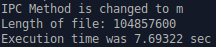
\includegraphics[width=5cm, height=1.2cm]{M_File}
\end{center}

Overall, the FIFO channels seemed to run a couple of seconds slower than the Message Queue and the Shared Memory Segment channels. The FIFO channel seems to run between 11 sec to 20 sec and the MQ and SHM channels seemed to run between 7 sec and 10 sec consistently. 

When splitting the file request (for 100MB) between multiple channels, the number of channels doesn't seem to affect the execution time to transfer the file. The times for each number of channels seem to vary between 10-20 sec and there isn't a very distinct number of channels that consistently gives a faster execution time. This is mainly because despite the number of channels created, the number of iterations needed to transfer the files is around the same number. Some channel numbers may have less or more iterations but overall the amount of iterations needed is about the same. If a lot of channels are created, then there could be a lot of iterations which could cause slow run time but for creating less than 50 channels won't create too much overhead that will cause a significant change in runtime. 

Link to youtube video: https://youtu.be/RSifn1YMKb4

\end{document}